\documentclass[12pt,pdftex,noinfoline]{imsart}

\RequirePackage[OT1]{fontenc}
\usepackage{amsthm,amsmath,amsfonts,natbib,mathtools,amssymb}
\RequirePackage{hypernat}
\usepackage[ruled,section]{algorithm}
\usepackage{algorithmic}
\usepackage{graphicx}
\usepackage{verbatim}
\usepackage{times}
\usepackage{hyperref}
\hypersetup{citecolor=MidnightBlue}
\hypersetup{linkcolor=MidnightBlue}
\hypersetup{urlcolor=MidnightBlue}
\usepackage{enumerate}
\usepackage{fullpage}
\usepackage{amssymb}
\usepackage{amsthm}
\usepackage{bbm}


\renewcommand{\d}{\mathrm{d}}
\newcommand{\E}{\operatorname{\mathbb E}}

\newcommand\numberthis{\addtocounter{equation}{1}\tag{\theequation}}

\DeclareMathOperator*{\argmin}{\arg\min}
\DeclareMathOperator*{\argmax}{\arg\max}

\numberwithin{equation}{section}
\newtheorem{theorem}{Theorem}[section]
\newtheorem{lemma}{Lemma}[section]
\newtheorem{corollary}{Corollary}[section]
\newtheorem{prop}{Proposition}[section]
\theoremstyle{remark}
\newtheorem{example}{Example}[section]
\newtheorem{remark}{Remark}[section]

\def\given{\,|\,}
\def\P{\mathbb{P}}
\def\E{\mathbb{E}}
\def\reals{\mathbb{R}}
\def\argmin{\mathop{\text{arg\,min}}}
\def\ones{\mathds{1}}
\def\indicator{}
\let\hat\widehat
\let\what\widehat
\let\tilde\widetilde
\let\epsilon\varepsilon

\setlength{\parskip}{0.5em}
\setlength{\parindent}{0pt}
\def\sfrac#1#2{#1/#2}

\begin{document}
\let\epsilon\varepsilon

\stepcounter{section}
{\large\bf Experiment: Underdetermined linear models}
\vskip10pt

In this experiment we simulate underdetermined linear models where $p > n$.
We generate $n$ data points $(X_i, y_i)$ where
$y_i = X_i^T \beta^* + w_i$ with $w_i$ an additive noise term. We then compute the minimum norm estimator
\begin{equation}
  \hat\beta = X^T (X X^T)^{-1} y
\end{equation}
The estimated model is corrupted to
\begin{equation}
  \eta = \hat\beta + z
\end{equation}
where $z_j \sim (1-\epsilon) \delta_0 +\epsilon Q$. The corrupted estimator is then repaired by performing median regression:
\begin{align}
  \tilde u &= \argmin \|\eta - X^T u\|_1 \\
  \tilde \beta &= X^T \tilde u
\end{align}

In the experiments shown below the design is sampled as $X_{ij} \sim N(0,1)$ and we take $\beta_j^* \sim N(0,1)$ and $Q = N(1,1)$. We take $n=50$ and $n=100$ and vary $p$ according to $p/n=200/j^2$ with
$j$ ranging from 1 to 9. The plots show the empirical probability of exact repair $\tilde\beta = \hat\beta$ as a function of $\epsilon$. Each point on the curves is the average repair success over $200$ trials.
The roughly equal spacing of the curves agrees with the theory, which indicates that $\sqrt{n/p}/(1-\epsilon)$ should be sufficiently small for successful repair.

\begin{figure}[ht]
  \begin{center}
    \begin{tabular}{cc}
      $n=50$ & $n=100$\\[-20pt]
      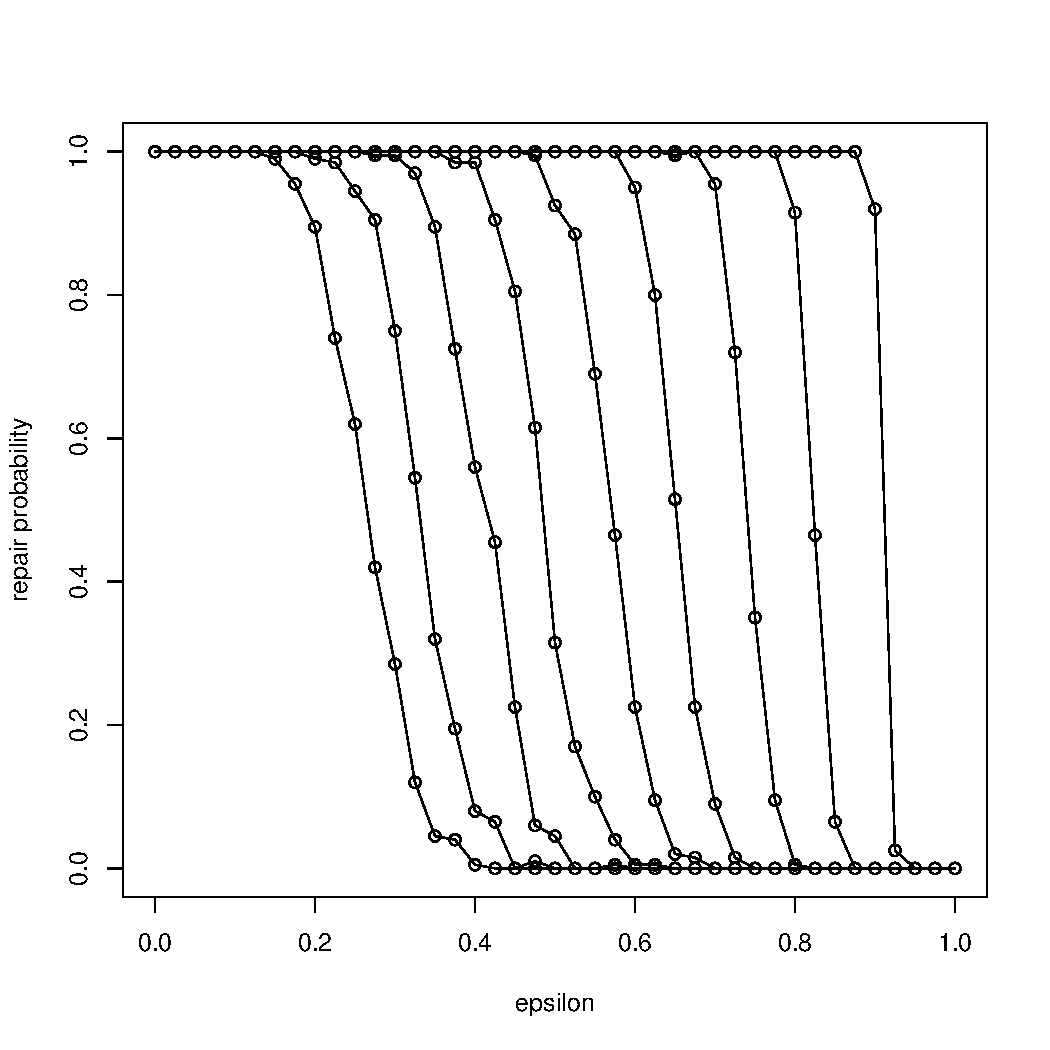
\includegraphics[width=.47\textwidth]{repair-n50} &
      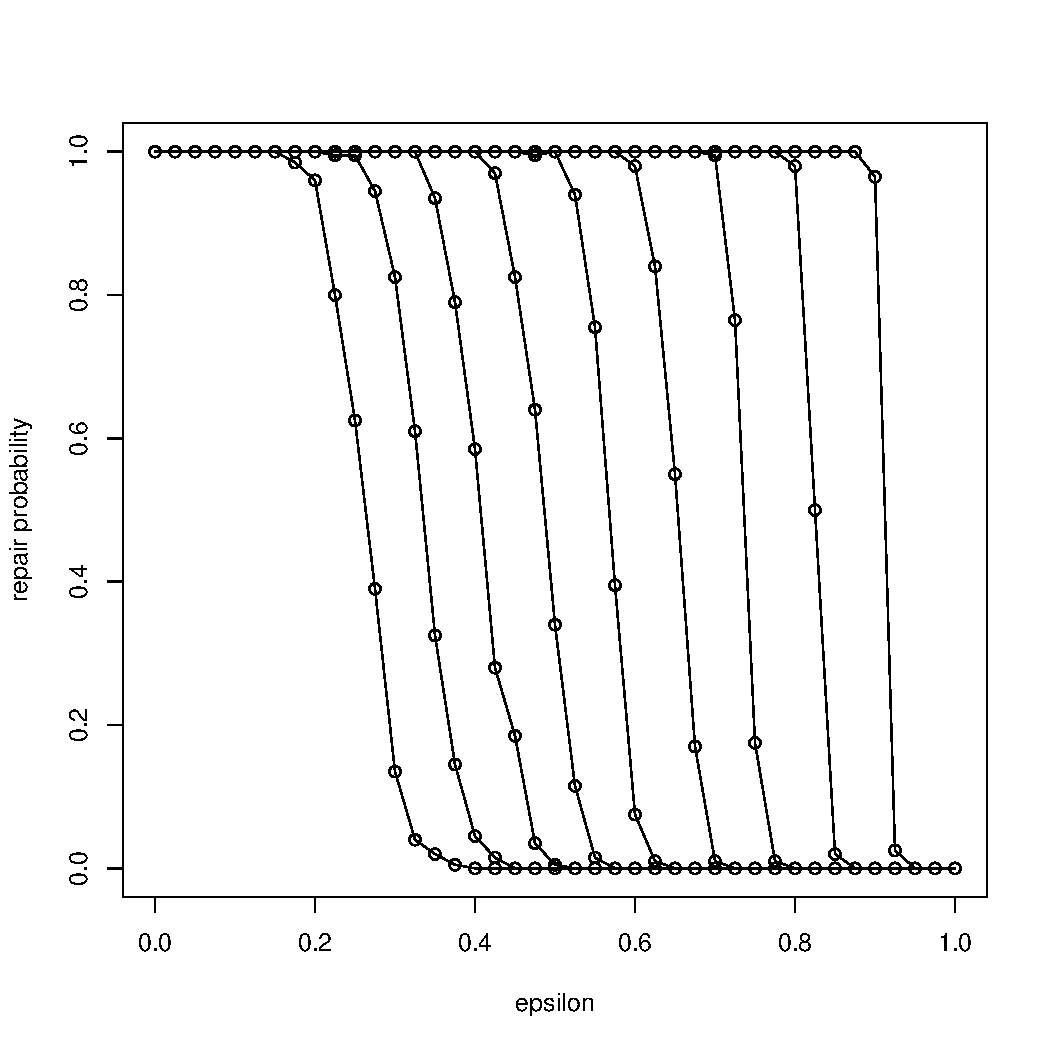
\includegraphics[width=.47\textwidth]{repair-n100}\\[-10pt]
    \end{tabular}
  \end{center}
\caption{Model repair for underdetermined linear models $y=X^T\beta + w$ with $p>n$. The plots show the probability of successful model repair for $n=50$ (left) and $n=100$ (right) with the model dimension $p$
varying as $p/n = 200 /j^2$, for $j=1,\ldots, 9$. Each point is an average over 200 trials.}
\end{figure}


\end{document}
